\newpage
\subsection{Topological Sorting / Ordering}
\begin{definition}[]{Topological Ordering}
    A \textbf{topological ordering} of a directed acyclic graph (DAG) $G = (V, E)$ is a linear ordering of its vertices such that for every directed edge $(u, v) \in E$, vertex $u$ comes before vertex $v$ in the ordering.
\end{definition}

\begin{properties}[]{Topological Ordering}
    \begin{itemize}
        \item A graph has a topological ordering if and only if it is a DAG.
        \item The ordering is not unique if the graph contains multiple valid sequences of vertices.
        \item Common algorithms to compute topological ordering:
              \begin{itemize}
                  \item \textbf{DFS-based Approach:} Perform a depth-first search and record vertices in reverse postorder.
                  \item \textbf{Kahn’s Algorithm:} Iteratively remove vertices with no incoming edges while maintaining order.
              \end{itemize}
    \end{itemize}
\end{properties}




\newpage
\subsection{Graph search}
\subsubsection{DFS}
\begin{definition}[]{Depth-First Search (DFS)}
    \textbf{Depth-First Search} is an algorithm for traversing or searching a graph by exploring as far as possible along each branch before backtracking.
\end{definition}

\begin{algorithm}
    \caption{Depth-First Search (Recursive)}
    \begin{algorithmic}[1]
        \Procedure{DFS}{$v$}
            \State \textbf{Mark} $v$ as visited
            \For{each neighbor $u$ of $v$}
                \If{$u$ is not visited}
                    \State \Call{DFS}{$u$}
                \EndIf
            \EndFor
        \EndProcedure
    \end{algorithmic}
\end{algorithm}

\begin{properties}[]{Depth-First Search}
    \begin{itemize}
        \item Can be implemented recursively or iteratively (using a stack).
        \item Time complexity: \tco{|V| + |E|}, where $|V|$ is the number of vertices and $|E|$ is the number of edges.
        \item Used for:
              \begin{itemize}
                  \item Detecting cycles in directed and undirected graphs.
                  \item Finding connected components in undirected graphs.
                  \item Computing topological ordering in a DAG.
              \end{itemize}
    \end{itemize}
\end{properties}


\subsubsection{BFS}
\begin{definition}[]{Breadth-First Search (BFS)}
    \textbf{Breadth-First Search} is an algorithm for traversing or searching a graph by exploring all neighbors of a vertex before moving to the next level of neighbors.
\end{definition}

\begin{algorithm}
    \caption{Breadth-First Search (Iterative)}
    \begin{algorithmic}[1]
        \Procedure{BFS}{$start$}
            \State \textbf{Initialize} queue $Q$ and mark $start$ as visited
            \State \textbf{Enqueue} $start$ into $Q$
            \While{$Q$ is not empty}
                \State $v \gets \textbf{Dequeue}(Q)$
                \For{each neighbor $u$ of $v$}
                    \If{$u$ is not visited}
                        \State \textbf{Mark} $u$ as visited
                        \State \textbf{Enqueue} $u$ into $Q$
                    \EndIf
                \EndFor
            \EndWhile
        \EndProcedure
    \end{algorithmic}
\end{algorithm}

\begin{properties}[]{Breadth-First Search}
    \begin{itemize}
        \item Implements a queue-based approach for level-order traversal.
        \item Time complexity: \tco{|V| + |E|}.
        \item Used for:
              \begin{itemize}
                  \item Finding shortest paths in unweighted graphs.
                  \item Checking bipartiteness.
              \end{itemize}
    \end{itemize}
\end{properties}

\begin{example}[]{DFS and BFS Traversal}
    \begin{center}
        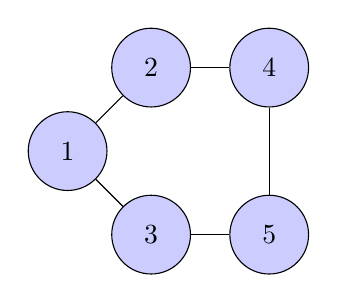
\begin{tikzpicture}[node distance=1.5cm, main/.style={circle, draw, fill=blue!20, minimum size=10mm, inner sep=0pt}]
            % Graph vertices
            \node[main] (1) {1};
            \node[main] (2) [above right of=1] {2};
            \node[main] (3) [below right of=1] {3};
            \node[main] (4) [right of=2] {4};
            \node[main] (5) [right of=3] {5};

            % Edges
            \draw (1) -- (2);
            \draw (1) -- (3);
            \draw (2) -- (4);
            \draw (3) -- (5);
            \draw (4) -- (5);
        \end{tikzpicture}
    \end{center}
    \textbf{DFS Traversal:} Starting at $1$, a possible traversal is $1 \to 2 \to 4 \to 5 \to 3$.\\
    \textbf{BFS Traversal:} Starting at $1$, a possible traversal is $1 \to 2 \to 3 \to 4 \to 5$.
\end{example}
